\chapter{Background and related work}
\label{chapter:background}

In this chapter I provide an overview and summary of the research that has been used by and influenced this work as well as covering similar research that has been performed. This includes a look at traffic engineering, reinforcement learning techniques, the advent of graph neural networks and other approaches to optimising networking using reinforcement learning.


\section{Traffic engineering}

\subsection{Intradomain routing}

The field of internet traffic engineering contains the problem of how to control and manage computer networks. One such problem is that of intradomain routing. Intradomain routing focusses on what paths data should take on a single network entirely controlled by one entity who generally has complete knowledge of the contents of the network and control over how the routing is to be managed (e.g. which protocol to use). An example of what we mean by a network controlled by one entity in this context is an autonomous system (AS). Autonomous systems can scale from the size of a small company to that of a large internet service provider (ISP).

The benefit of working inside and AS rather than the full internet is the complete knowledge and control which gives a lot more scope for achieving optimality concerning network control. For example, a network administrator can decide what their priorities are for the network and internally apply policy and routing that reflects those aims. Common aims are minimising latency between source and destination or minimising link utilisation to avoid congestion and packet loss. Examples of the most common protocols used for intradomain routing are RIP\cite{rfc2080} and OSPF\cite{rfc5340} which both minimise distance which generally equates to latency.

\subsection{Data-driven routing}

In the previous section intradomain routing was introduced along with the protocols commonly used for routing. These protocols have generally led to good performance and are deployed almost everywhere. However, they only take into account the structure of the network itself and not the traffic that goes over it. As different flows on the network can interfere with each other the data on the network can have an impact on the utility of the routing used. Therefore, if possible, taking into account the traffic conditions when performing routing can have a significant positive impact on performance (whether this be measured by latency, throughput or some other metric). This leads us to data-driven routing.

Data-driven routing seeks to make routing decisions that take into account the impact of traffic on the network. This is often to provide improved performance by reducing link congestion which is the utility which will be focussed on here.

\subsection{Multicommodity flow}
\label{section:multicommodity}

The problem of data-driven routing can in fact be modelled as a multicommodity flow problem. The multicommodity flow problem is simply a network flow problem with multiple demands between different source and sink nodes. It consists of a flow network $G(V,E)$ where each edge $(u,v) \in E$ has a capacity $c(u,v)$. Then we wish to place commodities $K_i = (s_i, t_i, d_i)$ on the network where $s_i$ is the source, $t_i$ is the sink and $d_i$ is the demand (the amount of data to pass between source and sink). Finally the following constraints must be satisfied:

\begin{enumerate}
    \item Flow on a link must not exceed its capacity:\\
    $\forall (u,v)\in E:\,\sum_{i=1}^{k} f_i(u,v)\cdot d_i \leq c(u,v)$
    \item Flow entering and exiting a node must be conserved:\\
    $\sum_{w \in V} f_i(u,w) - \sum_{w \in V} f_i(w,u) = 0 \quad \mathrm{when} \quad u \neq s_i, t_i$
    \item The entire flow of a commodity must exit its source:\\
    $\sum_{w \in V} f_i(s_i,w) - \sum_{w \in V} f_i(w,s_i) = 1$
    \item The entire flow of a commodity must be absorbed at the sink:\\
    $\sum_{w \in V} f_i(w,t_i) - \sum_{w \in V} f_i(t_i,w) = 1$
\end{enumerate}

In this framework we are able to specify any valid routing we wish (including splitting one flow across multiple routes) but importantly we can also optimise the routing under a given utility function using linear programming in polynomial time for a specified set of commodities (as long as we allow fractional flows)\cite{cormen2009introduction}. This in effect means optimal data-driven routing for reducing link congestion is solved except for the important fact that in most cases we do not know the traffic demands on a network in advance so the routing would always lag the commodities it was optimised for.

\subsection{Current approaches to reducing link congestion}

Current approaches to traffic engineering often rely on the use of software defined networking (SDN) which separates the control plane and data plane and allows for more complicated and custom routing schemes to be easily deployed\cite{doi:10.1002/sec.1737}. On top of these SDN systems many different methods have been used to achieve better network performance in the face of high traffic demands.

One such method are forms of oblivious routing\cite{Bansal2008} which seeks to reduce congestion on links in a network without the knowledge of what the traffic demands are. Early examples of approaches are that of R\"acke\cite{racke2002minimizing} who showed that it is possible to have an optimal oblivious routing and Azar\cite{azar2004optimal} who proved that this can be calculated in polynomial time. Since then, small, incremental improvements have been made, improving calculation time or allowing for different utility functions to be specified\cite{kodialam2008advances}.

However, it is still possible to do better than oblivious routing if you have some knowledge of the traffic. One seminal work in this area is SMORE\cite{kumar2018semi} which combines oblivious routing and adaptive sending rates to improve reliable network performance under all kinds of operating conditions.

On will notice that while all of these methods do successfully improve network performance in the sense of reducing link congestion, they are all fundamentally limited by their knowledge (or lack thereof) of the current operating conditions of the network they are creating a routing strategy for. 


\section{Machine learning}

\subsection{Reinforcement learning}

Reinforcement learning (RL)\cite{sutton2018reinforcement} is a subsection of machine learning the third of the three paradigms, the other being supervised and unsupervised learning. It is concerned with training agents to take actions in some specified environment and achieve a goal in that environment as can be seen in Figure~\ref{fig:reinforcement_learning}. Commonly the agent makes choices using a neural network which is trained using any one of multiple algorithms designed for this purpose (all with different trade-offs). RL is powerful as it does not require an analytical model of the environment being used as it is able to find out how to act through exploration alone. RL has been used successfully in many fields approaching many different problems such as in robotics\cite{}, game-playing\cite{}, \todo{fill in these citations} and general optimisation with one recent success being playing board games to a super-human level with AlphaZero\cite{Silver1140}.

\begin{figure}
    \centering
    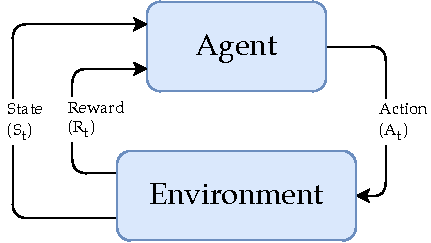
\includegraphics[width=0.5\textwidth]{figures/reinforcement_learning.pdf}
    \caption{The structure of a reinforcement learning problem: the interaction of agent and environment}
    \label{fig:reinforcement_learning}
\end{figure}

Formally, a RL problem is generally framed with the environment modelled as a finite Markov decision process (MDP) which can be defined as the 4-tuple $(S, A, P_a, R_a)$ where:
\begin{itemize}
    \item $S$ is a finite set of states
    \item $A$ is a finite set of actions
    \item $P_a(s,s')$ is the probability that action $a$ in state $s$ at time $t$ will lead to state $s'$ at time $t + 1$
    \item $R_a$ is the reward received after transitioning from state $s$ to state $s'$, due to taking action $a$
\end{itemize}

With a MDP defined as our environment it is then necessary to create an agent to interact with it. Generally such an agent is implemented by a policy which will return an action given an observation (which is a set of features probabilistically derived from the current state of the environment). This policy can take many forms but in deep RL as used in this research it takes the form of a neural network.

The final piece of the RL puzzle is a way to make the policy act how we want it to (or formally to maximise the reward it can achieve in an episode). Again, there are multiple ways to do this. One such method is the policy gradient method with the first prominent example being REINFORCE\cite{williams1992simple}. One branch of this to have gained traction in particular are actor-critic algorithms. These have two main parts:

\begin{itemize}
    \item The \emph{critic} which updates the value function ($V(s)$, the expected reward from a given state) given feedback from the environment.
    \item The \emph{actor} which updates the policy ($\pi(a|s)$, the probability of choosing an action in a state) using feedback from the critic.
\end{itemize}

PPO\cite{schulman2017proximal} is an example of an actor-critic algorithm that achieves good sample efficiency and performance while maintaining a fairly simple implementation (relative to similar algorithms). This is mainly because of how it restricts the maximum size of policy updates. It has had notable successes such as beating world champions in a live game of Dota 2\cite{openai2019dota}.

\subsection{Graph neural networks}
\label{section:graph_neural_networks}

Graph neural networks (GNNs)\cite{gori2005new,scarselli2008graph} are a form of neural network that has gained considerable 
traction over the last few years. This is because, in the same way that convolutional neural networks (CNNs) have been used with much success on images as pixels form a grid and are often related to their neighbouring pixel, many other datasets are graph structured with relations to neighbouring nodes being an important part of this structure. GNNs effectively allow us to generalise the CNN model onto graphs. \todo{give some example uses} There are many different types of GNN with different trade-offs as described in countless surveys of the subject\cite{zhou2018graph,Wu_2020}.

Possibly the most general model, allowing for restrictions to define the different subtypes of graph network is that proposed by Battaglia et al.\cite{battaglia2018relational}. They propose that combinatorial generalisation is crucial to learning and that this relies on the integration of structured and unstructured approaches. All networks contain some level of structure leading to relational inductive biases but it is only graph networks that give fine-grained control over these biases to fully harness the structure present in the problem being solved and without implying structure that is not present.

The model presented by Battaglia et al.\ defines a Graph Network (GN) Block which takes as input a graph and returns a graph. Here a graph is defined to be the 3-tuple $G = (\bm{u}, V, E)$ where $\bm{u}$ is a global attribute vector, $V = \{\bm{v}_i\}_{i=1:N^v}$ is the set of vertex attribute vectors, and $E = \{(\bm{e}_k, r_k, s_k)\}_k=1:N^e$ is the set of edge attribute vectors and their source and destination vertices.

The graph block itself computes over an input graph as shown in Algorithm~\ref{algorithm:graph_block}. This algorithm contains three $\phi$ functions which update attribute information and three $\rho$ functions which pool attribute information to be used in the updates. It is the coefficients in these functions that are learn and the ability to change the operations that these functions perform that allows for the flexibility to implement many different types of GNN.\todo{insert Graph Network Block Diagram maybe?}

\begin{algorithm}[t]
\small
\begin{algorithmic}
\Function{GraphNetwork}{$E$, $V$, $\mathbf{u}$}
    \For {$k\in \{1\ldots{}N^e\}$}
        \State $\mathbf{e}_k^\prime\gets \phi^e\left(\mathbf{e}_k, \mathbf{v}_{r_k}, \mathbf{v}_{s_k}, \mathbf{u} \right)$
        \Comment{1. Compute updated edge attributes}
    \EndFor
    \For {$i\in \{1\ldots{}N^n\}$}
        \State \textbf{let} $E'_i = \left\{\left(\mathbf{e}'_k, r_k, s_k \right)\right\}_{r_k=i,\; k=1:N^e}$
        \State $\mathbf{\bar{e}}'_i \gets \rho^{e \rightarrow v}\left(E'_i\right)$
        \Comment{2. Aggregate edge attributes per node}
        \State $\mathbf{v}'_i \gets \phi^v\left(\mathbf{\bar{e}}'_i, \mathbf{v}_i, \mathbf{u}\right)$
        \Comment{3. Compute updated node attributes}
    \EndFor
    \State \textbf{let} $V' = \left\{\mathbf{v}'\right\}_{i=1:N^v}$
    \State \textbf{let} $E' = \left\{\left(\mathbf{e}'_k, r_k, s_k \right)\right\}_{k=1:N^e}$
    \State $\mathbf{\bar{e}}' \gets \rho^{e \rightarrow u}\left(E'\right)$
    \Comment{4. Aggregate edge attributes globally}
    \State $\mathbf{\bar{v}}' \gets \rho^{v \rightarrow u}\left(V'\right)$
    \Comment{5. Aggregate node attributes globally}
    \State $\mathbf{u}' \gets \phi^u\left(\mathbf{\bar{e}}', \mathbf{\bar{v}}', \mathbf{u}\right)$
    \Comment{6. Compute updated global attribute}
    \State \Return $(E', V', \mathbf{u}')$
\EndFunction
\end{algorithmic}
\caption{Steps of computation in a full GN block. (Taken from \cite{battaglia2018relational})}
\label{algorithm:graph_block}
\end{algorithm}


\section{Approaches to routing using reinforcement learning techniques}

There have thus far been multiple approaches to network-related problems using machine learning and especially reinforcement learning techniques. There is a growing body of work covering areas from routing to deep packet inspection. Specifically in the area of routing, there has been reinforcement research for quite a while with an early seminal paper introducing the idea of Q-routing in 1994\cite{boyan1994packet} which attempts to use distributed on-device agents to route packets so as to minimise delay. Many pieces of work have followed a similar vein gradually improving on Q-routing with ever more complex policies\cite{you2019toward,Ali2019HierarchicalDD}.

A separate issue is the traffic engineering problem where one can make global decisions for a large scale network (such as an autonomous system) on a longer timescale. In this area there has recently been one major work: ``Learning to Route with Deep RL''\cite{valadarsky2017learning} which is the paper who's research our work seeks to extend and improve. The paper introduces the problem of knowing the history of traffic demands for a given network and using it along with a neural network to predict what routing should be used on the network in the next timestep to minimise link over utilisation. This is performed using reinforcement learning with a novel translation from action to routing.

Similarly, another paper: ``A Deep-Reinforcement Learning Approach for Software-Defined Networking Routing Optimisation''\cite{stampa2017deep} sought to use reinforcement learning to find good routes for a given traffic matrix. However, this means that the matrix must be known in advance and we already have deterministic algorithms than can find optimal routings given a traffic matrix. Also, within the last few months there has been some other work on optimising routing, this time looking at link utilisation and using GNNs\cite{Sawada2020NetworkRO}. However, it learns to cope with the current traffic flow as it is occurring and is distributed rather than centralised.
